% =====================================================================================================================
\section{Results}
\label{sec:results}

\subsection{Reviewers name the wrong number but keep the score}
\label{sec:reviewers}

\begin{figure}[t]
  \centering
  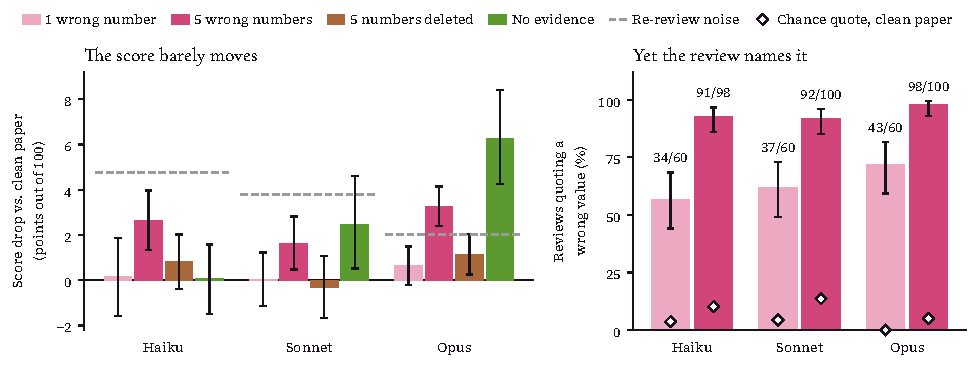
\includegraphics[width=\linewidth]{figures/fig2_reviewers.pdf}
  \caption{LLM reviewers see planted wrong numbers but barely lower their scores. Left: mean drop in the 0--100
  review score from the clean paper for each edited version, per reviewer, over 60 post-cutoff arXiv papers. The
  versions shift one prose number so it contradicts its table (1 wrong), shift five (5 wrong), delete the same five
  (5 deleted), or remove the experiments section and every table (no evidence). The number above each bar is its
  mean; error bars are 95\% bootstrap intervals over papers; the dashed line is the mean difference between two
  reviews of the same clean paper. Right: share of reviews whose summary, weaknesses, or questions quote at least one planted
  wrong value, with 95\% Wilson intervals; diamonds give the share of clean-paper reviews that quote the same
  values by coincidence. Read the panels together: the reviewers find the errors (right), and the score hardly reflects them
  (left).}
  \label{fig:reviewers}
\end{figure}

LLM reviewers find wrong numbers and then score the paper as if they had not. When five prose numbers contradict the
paper's own tables, more than 9 in 10 reviews from every reviewer quote at least one wrong value in their summary,
weaknesses, or questions. On the clean paper, about 1 in 10 reviews quote such a value by coincidence
(Fig.~\ref{fig:reviewers}, right). Yet those five errors lower the score by less than 3.5 points out of 100. For Haiku and Sonnet this is less than the
4 to 5 points by which two reviews of the same unchanged paper differ; for Opus, whose reviews vary less, it is about 1
point more. A single wrong number costs almost nothing (Fig.~\ref{fig:reviewers}, left).

Deleting the same five numbers costs slightly less than making them wrong, for all three reviewers. A wrong number
therefore costs a little more than a missing one, and the cost of deleting them stays within the difference between
two reviews of the same paper for every reviewer. Removing the evidence altogether separates the reviewers: Opus loses about 6 points when the
experiments and every table are gone, Sonnet loses about 2.5, and Haiku loses nothing (Appendix Table~\ref{tab:killa}).
The reviewers are able to see errors. In a pilot where the judge compared the clean and the edited paper side by side,
it preferred the clean one in most pairs, because it compared the two versions and checked the arithmetic
(Appendix~\ref{app:killa}). A single review has no clean copy to compare against, and its score does not reflect the
errors that its own text points out.

This matters for a writing loop that keeps a revision only when the score rises. The score says almost nothing about
whether the paper's numbers are right. For reviewers smaller than Opus, it also says little about whether the numbers
are there at all.

\begin{finding}
The reviewer cannot serve as the number check. A reviewer reads the wrong number, quotes it, and returns nearly the
same score, so a loop that optimizes the score never learns that the number was wrong.
\end{finding}

\subsection{Agents compute their new numbers, and recomputation finds the few wrong ones that lookups miss}
\label{sec:checkers}

\begin{table}[t]
  \centering
  \caption{Errors caught and false alarms per checker on a random sample of 300 numbers that writers added or changed
  under reviewer pressure. Left: against the two-model blind labels (13 agreed errors, 193 correct numbers). Right:
  against the human recomputation of a 122-row packet (16 human-found errors). Human false alarms are counts on that
  packet, which includes every row a checker flagged, not rates on all numbers. Matched audits use the probability
  cutoff at which the audit flags no more correct numbers than recompute does on the two-model labels. The two-model
  audit row is the ground truth of the left block and is scored on the right block only. Bold marks the best single
  checker per column.}
  \label{tab:checkers}
  \small
  \begin{tabular}{@{}lcccc@{}}
    \toprule
    \rowcolor{headgray}
    & \multicolumn{2}{c}{Two-model labels} & \multicolumn{2}{c}{Human labels} \\
    \rowcolor{headgray}
    Checker & \makecell{Errors caught\\(of 13)} & \makecell{Correct flagged\\(of 193)} &
    \makecell{Errors caught\\(of 16)} & \makecell{False\\alarms} \\
    \midrule
    Lookup gate                          & 1           & 22         & 3           & 8 \\
    \ours Recompute (\tool{})            & \best{12}   & 24         & \best{14}   & 27 \\
    Sonnet audit agent, flags only       & 4           & \best{0}   & 4           & \best{0} \\
    Sonnet audit agent, matched          & 8           & 18         & 9           & 10 \\
    Opus audit agent, matched            & 11          & 16         & 12          & 10 \\
    Opus audit agent, $p \ge 50$         & 11          & \best{0}   & 9           & 3 \\
    \midrule
    Two-model blind audit                & \multicolumn{2}{c}{\textit{reference labels}} & 10 & 3 \\
    Recompute or Opus audit, matched     & 13          & 36         & 16          & 31 \\
    \bottomrule
  \end{tabular}
\end{table}

\begin{figure}[t]
  \centering
  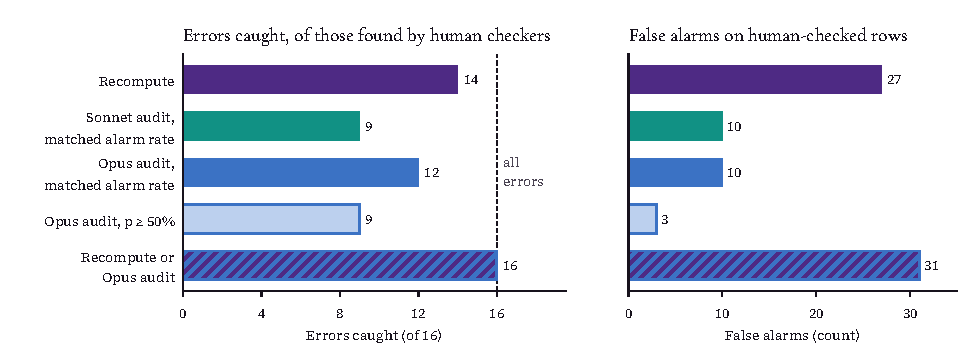
\includegraphics[width=0.78\linewidth]{figures/fig3_checkers.pdf}
  \caption{Recompute and an Opus audit agent each catch most human-found errors, and they miss different ones. Each
  bar is one checker on the human-checked packet: errors caught, of the 16 that the human recomputation found (left),
  and false alarms, the numbers flagged that the human found correct (right). Matched audits flag no more correct
  numbers than recompute on the two-model labels; ``Opus audit $p \ge 50$'' uses a fixed cutoff instead. ``Recompute
  or Opus'' flags a number when either checker does. False alarms are counts on a packet enriched for flagged rows.}
  \label{fig:checkers}
\end{figure}

Writers revising under reviewer pressure compute new results from the data instead of inventing them. For example, a
writer recomputes a full column from per-question files that the repository never summarized, and it adds seed means,
intervals, and caveats. Almost all of these numbers are right: on the random sample, about 4\% of the numbers writers
added are wrong by both audits. The wrong ones are small and plausible (Table~\ref{tab:natural}): a rounding slip
after subtracting rounded values, an effect given in the wrong unit, a value copied from an out-of-date note that the
data contradicts, or a rate over a different denominator.

\begin{table}[t]
  \centering
  \caption{Errors that writing agents made on their own, with the value a human recomputed from the raw files.
  These are rows of the human-checked packet, one per kind of slip. The last column says whether the recompute check
  flagged the number; the two it missed have recipes that compute a neighboring quantity.}
  \label{tab:natural}
  \small
  \setlength{\tabcolsep}{4pt}
  \begin{tabular}{@{}llllc@{}}
    \toprule
    \rowcolor{headgray}
    Kind of slip & Printed & Data gives & What happened & Recompute \\
    \midrule
    Rounding           & $-3.0$\%   & $-3.05$\%  & Smallest field gain, rounded toward zero & \cmark \\
    Rounding           & $+15.1$    & $15.04$    & Upper end of a paired interval           & \cmark \\
    Wrong unit         & 48 points  & 24 points  & 48 episodes of 200, printed as percentage points & \cmark \\
    Other denominator  & 19.6\%     & 19.7\%     & 88 answers over 446 items, where a nearby count is 438 & \xmark \\
    Other population   & $+6.8$     & $5.9$      & A rate reduction taken over a different set of runs & \cmark \\
    Miscount           & 53.6\%     & 54.0\%     & Accuracy over the parseable records of one model & \cmark \\
    Neighboring quantity & 14 series & 12 series & Two of the 14 entries are variants of existing series & \xmark \\
    \bottomrule
  \end{tabular}
\end{table}

Because the new numbers are fresh computations, a lookup of stored values cannot tell right from wrong. On realistic
edits, more than 8 in 10 numbers our lookup gate flagged were correct new analyses and fewer than 1 in 10 were errors, and on the random sample it caught 1 of the
13 agreed errors (Table~\ref{tab:checkers}). A trace of the finished paper does no better, for a different reason. A
real repository holds thousands to hundreds of thousands of values, so when we shifted every decimal in a paper, most
of the shifted numbers still found a plausible match (Appendix Table~\ref{tab:trace}). Recomputing the writer's own
recipe asks a narrower question, namely whether this computation on this data gives this number. It caught 12 of the
13 agreed errors while flagging correct numbers at about the same rate as the lookup gate.

The human recomputation confirms this without relying on any model. The humans found 16 errors: 10 of the 13 agreed ones,
4 of the 9 disputed ones, and 2 that both model audits had called correct. Recompute caught 14 of the 16, including
both that the model auditors had missed, and none of the 76 numbers that recompute and the model audits had both
passed was flagged by a human. Its two misses share one cause: a recipe computed a plausible value
for a slightly different quantity, such as a count that includes variants or a rate with another denominator. This is
the known blind spot of any check that trusts the writer's statement of what a number means. It is also why audits
must be blind. An earlier audit that could read the recipes tended to accept them, and a blind re-audit overturned 17
of its 40 errors. Each was a case where a plausible recipe computed a neighboring quantity (Appendix~\ref{app:audit}).

An audit agent is the obvious alternative, and a strong one does well. When asked only to flag numbers, a Sonnet audit
flags few and finds few errors. When asked for a probability on every number, with the cutoff set to recompute's
alarm rate, an Opus audit catches about as many human-found errors as recompute, with fewer false alarms on the packet
(Fig.~\ref{fig:checkers}). The two checkers fail on different numbers. Recompute misses the recipe that computes a
neighboring quantity. The Opus audit misses numbers it never lists and rounding slips it lets pass, such as a gain of
$-3.05$ printed as $-3.0$ that it rated at a 5\% chance of being wrong. Together they miss none of the human-found
errors. What recompute adds is where and how it runs. It runs at the edit rather than on a finished paper, it is
deterministic, it needs no model call per check, and it has the value from the data ready to send back to the agent.

\begin{finding}
A number check must recompute the value. Agents under review write new analyses, so matching printed numbers against
stored values flags correct work and misses the errors. Rerunning the writer's own recipe catches nearly all of them,
and a strong audit catches the ones it misses.
\end{finding}

\subsection{A check works when it runs by itself at the edit}
\label{sec:placement-results}

\begin{figure}[t]
  \centering
  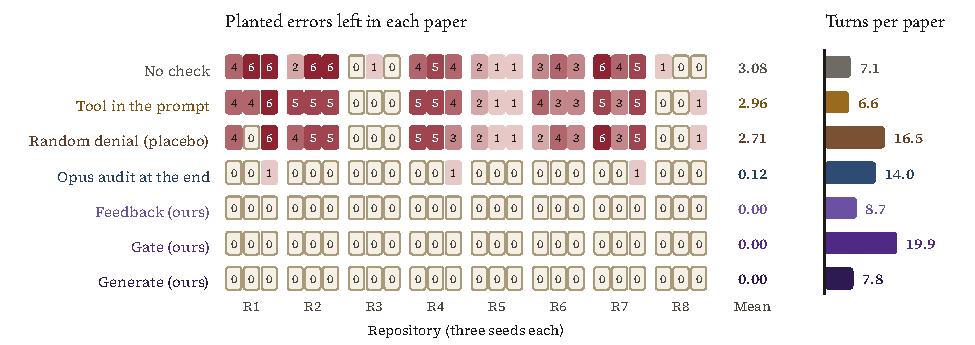
\includegraphics[width=\linewidth]{figures/fig5_study.pdf}
  \caption{The placement study, paper by paper. Left: each cell is one paper (8 repositories, three seeds each)
  revised under one placement of the check; the number and the shade give the planted errors still in the paper at
  the end, of up to six (four in R3). The three placements that run at the edit without being asked clear every
  paper. The prompted tool and the random-denial placebo look like no check at all. Right: mean agent turns per
  paper. Feedback and generate cost about as many turns as no check; the gate costs more than twice as many.}
  \label{fig:study}
\end{figure}

\begin{table}[t]
  \centering
  \caption{Where the check sits: the placement study on 8 repositories $\times$ 3 seeds (24 papers per arm, 138
  planted errors per arm, 96 of them flattering). Planted errors left are mean $\pm$ sd over papers, of up to six;
  the next two columns are totals over the arm. Correct turned wrong counts numbers whose original recipe no longer
  reproduces them (13 of the 14 are one disputed model count in one paper). The fresh review is one new Sonnet review
  of the final paper on the 0--100 scale; the planted draft scored 25.8. Denials count edits refused by the gate or the placebo; the other arms never refuse an edit. Shaded rows are \tool{}'s automatic modes.
  $\dagger$ marks arms that leave fewer errors than the prompted tool after Holm correction.}
  \label{tab:placement}
  \small
  \setlength{\tabcolsep}{4pt}
  \begin{tabular}{@{}lccccccc@{}}
    \toprule
    \rowcolor{headgray}
    Placement & \makecell{Planted errors\\left / paper $\downarrow$} & \makecell{Corrected\\(of 138) $\uparrow$} &
    \makecell{Correct turned\\wrong $\downarrow$} & \makecell{New numbers\\/ paper} & \makecell{Turns\\/ paper} &
    \makecell{Denials\\/ paper} & \makecell{Fresh\\review} \\
    \midrule
    No check                          & 3.08 $\pm$ 2.21 & 61  & 0  & 30.6 & 7.1  & 0.0 & 27.0 \\
    Tool and rules in the prompt      & 2.96 $\pm$ 2.07 & 67  & 0  & 9.8  & 6.6  & 0.0 & 26.8 \\
    Random denial, matched rate       & 2.71 $\pm$ 2.16 & 73  & 0  & 12.1 & 16.5 & 2.3 & 26.1 \\
    End-of-session Opus audit         & 0.12 $\pm$ 0.34 & 135 & 14 & 38.9 & 14.0 & 0.0 & 27.2 \\
    \midrule
    \ours Feedback after each edit$^\dagger$ & \best{0.00 $\pm$ 0.00} & 137 & 0 & 13.4 & 8.7  & 0.0 & 27.0 \\
    \ours Blocking gate$^\dagger$            & \best{0.00 $\pm$ 0.00} & \best{138} & 0 & 12.6 & 19.9 & 2.9 & 26.9 \\
    \ours Generate mode$^\dagger$            & \best{0.00 $\pm$ 0.00} & \best{138} & 0 & 12.8 & 7.8  & 0.0 & 27.5 \\
    \bottomrule
  \end{tabular}
\end{table}

A check is reliable only when the agent does not have to remember to call it. Every placement that runs the check by
itself (feedback after each edit, the blocking gate, and generate mode) left no planted error in any of the 24 papers
and laundered none (Fig.~\ref{fig:study}, Table~\ref{tab:placement}). Offering the same check in the prompt, with the
same rules, did no better than no check at all. Writers without any check still corrected some planted errors while
they answered the review, which is why the top rows are below six. The automatic placements removed the rest.

\paragraph{Refused edits alone do not remove errors.}
Being refused makes an agent slow down and look again, and that alone might remove errors. The placebo arm tests
this. It refuses edits that touch numbers as often as the gate does, at random and with a generic message, and it
keeps the gate's rule against editing the paper through the shell. Its papers end with as many planted errors as
papers with no check. The gate adds the check and the value it returns, and the placebo has neither.

\paragraph{A reason to keep the error does not change the outcome.}
Errors that make the paper's own method look better are the ones an agent optimizing a reviewer might defend, so four
of the six planted errors in every paper are of this kind. Without an automatic check, the writer left close to half
of them in place, and about seven in ten of the neutral slips. With feedback, the gate, or generate mode,
none of either kind remained (one planted number was deleted; every other one was corrected). No arm fitted a recipe to a wrong number.

\paragraph{Blocking adds nothing over feedback, and costs turns.}
For this writer, a message after the edit was enough. The gate reached the same outcome as feedback but used more
than twice the turns, because a denied edit has to be proposed again. Generate mode was as clean as feedback and used
the fewest turns of the three. Feedback is therefore \tool{}'s default.

\paragraph{The recipe rule changes how much the agent writes.}
When the reviewer asked for new analyses, writers without the rule added about 31 numbers per paper. Writers that had
to leave a recipe added 10 to 13, and each of these follows from the data. The rule has this effect even when it only
sits in the prompt, where it does not remove the planted errors. With the rule, the writer adds fewer new numbers, but
we can be sure each one follows from the data. We consider this the right trade for a results section, and we report
it so that users can decide.

\paragraph{An audit at the end comes close, but costs more.}
An Opus audit of the finished paper, with its flags sent back to the writer, removed nearly all planted errors. It
also changed numbers that their recipes showed to be right, most of them in one paper where the audit and the recipe
disagree on which models to count. In addition, it costs a second, much larger model run on every draft. Fixing the errors did
not raise the score of a fresh reviewer, whose scores were the same in every arm. This is the reviewer result of
Section~\ref{sec:reviewers} seen from the writer's side.

\begin{figure}[t]
\begin{card}[darkbar]{1\quad The paper before the session (repository R6, seed 0): a planted flattering error}
\begin{lstlisting}[style=plain]
... a joint frame-plus-gradient probe has point estimates above the threshold on WikiText-2
(+1.57\src{joint_wt_min_abstract} to +2.33\pp) and below it on a public corpus
(+0.80\src{joint_pub_min_abstract} to +0.99\pp).
\end{lstlisting}
\end{card}
\begin{card}[nwpurple]{2\quad Hook to agent, after the agent's first edit (feedback mode)}
\begin{lstlisting}[style=plain]
Feedback only, your edit was kept. 4 number(s) could not be recomputed from the repository's data:
- +0.80 (line 21, key joint_pub_min_abstract): recipe gives 0.749682, which does not round to
  +0.80 at the printed precision. ...
- +0.15 (line 138, key margin_seed48): recipe gives 0.1433, which does not round to +0.15 ...
- +0.6692 (line 161, key mean_fwd_rep): recipe gives 0.669, which does not round to +0.6692 ...
- +0.75 (line 266, key fwd_gate_open_max): recipe gives 0.767412, which does not round to +0.75 ...
\end{lstlisting}
\end{card}
\begin{card}[teal]{3\quad The paper after the session: all six planted errors corrected, no recipe changed}
\begin{lstlisting}[style=plain]
... and below it on a public corpus (+0.75\src{joint_pub_min_abstract} to +0.99\pp).

@source("joint_pub_min_abstract", means="smallest paired joint point effect (pp) over the three
        open-gradient public-corpus cells ...")
def joint_pub_min_abstract():
    return min(_joint_paired("d1_puboff_"))
\end{lstlisting}
\end{card}
\caption{One session from the placement study, as logged. The planted error raises a result of the paper's own
method from $+0.75$ to $+0.80$. After the writer's first edit, the hook reran every
recipe and listed the numbers that no longer follow, each with the value its recipe gives; the two errors not
listed here were corrected by that same edit. The writer changed the printed numbers and left the recipes alone.
Messages are shortened where marked.}
\label{fig:case}
\end{figure}

Figure~\ref{fig:case} shows what this looks like inside one session. The message is short. It names the line and the
key and gives the value from the data. The agent does not need to be persuaded. It needs to be told, at a moment
when fixing the number takes a single edit.

\begin{finding}
Where a check runs decides whether it works. The same recompute check removes every planted error when it runs by
itself at the edit. For this writer, it removes no more than no check when it waits to be called. Refusing edits
without a check does no better, and blocking adds nothing over a message.
\end{finding}

% ---------------------------------------------------------------------------------------------------------------------
\subsection{The outcome survives an instruction to keep the results, and a change of writer}
\label{sec:extensions}

The placement study leaves two open questions. First, its writer had no reason to keep any particular number, so the
gate never had to overrule the writer. Second, every writer was Sonnet. We tested each question in turn on the same
24 papers (Fig.~\ref{fig:extend}; Appendix~\ref{app:extensions}).

\begin{figure}[t]
  \centering
  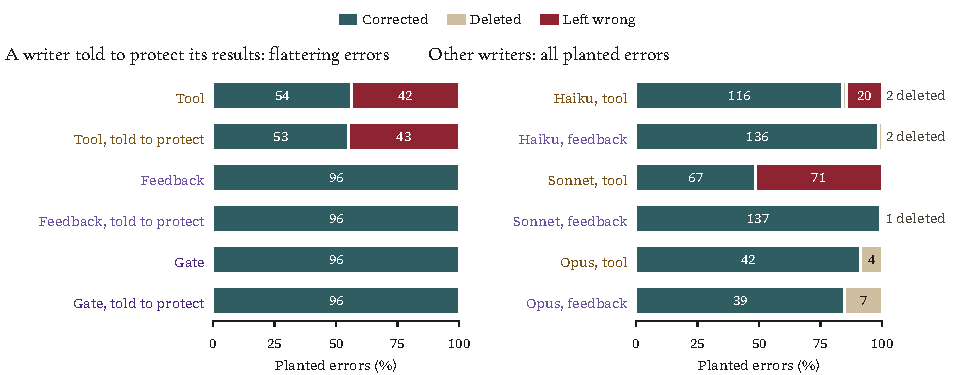
\includegraphics[width=\linewidth]{figures/fig6_extend.pdf}
  \caption{Two extensions of the placement study on the same papers. Left: what became of the flattering planted
  errors (96 per arm) when the writer's prompt tells it not to weaken the paper's headline results, next to the same
  arms without that instruction. Right: what became of all planted errors for a Haiku, a Sonnet, and an Opus writer,
  with the check offered in the prompt and with feedback after each edit (138 per arm over 24 papers; the Opus arms
  cover one seed, 46 errors over 8 papers). Counts are printed inside the segments, or beside the bar when a segment is too thin to hold one. No session laundered an error or
  moved a planted number to a third value.}
  \label{fig:extend}
\end{figure}

\paragraph{A recomputed value outweighs an instruction to keep the result.}
We added a note from the lead author to the writer's prompt: the headline results must not be weakened, and every
number about our own method must stay at least as favorable as it is in the draft. Correcting a flattering error now
means disobeying the note. Under feedback and under the gate, the writer corrected every one of them anyway. It
deleted none and fitted no recipe to a wrong number. The note did not change the offered-tool arm either, which left the same share of
flattering errors with it as without it. Blocking again had nothing to add over a message, and the gate reached the
outcome of feedback with more than twice the turns (Appendix Table~\ref{tab:extdefend}). An agent that sees the
value its own recipe gives accepts that value, even after being told to keep its results.

\paragraph{What an offered check removes depends on the writer; what an automatic one removes does not.}
With the check only offered, the three writers ended with very different results. Sonnet left about half of the
planted errors, Haiku about one in seven, and Opus none. The two writers that left fewer also spent five to six times
as many turns on each paper as Sonnet did. We did not record whether they called the check, and we ran no arm without
it for them. We therefore cannot separate the effect of the offer from the effect of the writer. With feedback after
each edit, this question does not arise: no writer left a planted error (Appendix Table~\ref{tab:extwriters}). A user
rarely knows in advance how a writer will behave or how much effort it will spend on a given revision. A check that
runs at the edit does not require the user to know.

\begin{finding}
The check that runs by itself removed every planted error for writers of three sizes and for a writer told to keep
its results. How much an offered check removes depends on the writer.
\end{finding}


\subsection{Reviewer pressure did not produce hollow gains}

We expected writers that optimize a reviewer's score to gain points while their numbers drifted away from the
evidence. This did not happen. Inside the loop, the Haiku writer's score rose by about 6 points, but fresh reviews of the starting and final
drafts by the loop's reviewer and by a held-out Opus reviewer show no reliable gain for any writer or arm once the
best-of-three selection is removed (Appendix Table~\ref{tab:rescore}). Confirmed error rates per number, which are lower bounds, stayed small and did
not rise consistently under the reviewer (the reviewed Haiku writer erred less often than its control); reviewed papers
simply contained more numbers and so ended with more errors in absolute terms (Appendix Table~\ref{tab:perarm}).
When a repository of real results was available, reviewer pressure made writers compute more numbers, and it did not
make them invent more. An edit-time check is therefore needed because any revision makes errors, and not because a
reviewer rewards them.
